%%%%%%%%%%%%%%%%%%%%%%%%%%%%%%%%%%%%%%%%%%%%%%%%%%%%%%%%%%%%%%%%%%%%%%%%%%%%%%%%%%%%%%%%%%%%%%%%%%%%%%%%%%%%%%%%%%%%%%%%%%%%%%%%%%%%%%%%%%%%%%%%%%%%%%%%%%%
% This is just an example/guide for you to refer to when submitting manuscripts to Frontiers, it is not mandatory to use Frontiers .cls files nor frontiers.tex  %
% This will only generate the Manuscript, the final article will be typeset by Frontiers after acceptance.
%                                              %
%                                                                                                                                                         %
% When submitting your files, remember to upload this *tex file, the pdf generated with it, the *bib file (if bibliography is not within the *tex) and all the figures.
%%%%%%%%%%%%%%%%%%%%%%%%%%%%%%%%%%%%%%%%%%%%%%%%%%%%%%%%%%%%%%%%%%%%%%%%%%%%%%%%%%%%%%%%%%%%%%%%%%%%%%%%%%%%%%%%%%%%%%%%%%%%%%%%%%%%%%%%%%%%%%%%%%%%%%%%%%%

%%% Version 3.4 Generated 2022/06/14 %%%
%%% You will need to have the following packages installed: datetime, fmtcount, etoolbox, fcprefix, which are normally inlcuded in WinEdt. %%%
%%% In http://www.ctan.org/ you can find the packages and how to install them, if necessary. %%%
%%%  NB logo1.jpg is required in the path in order to correctly compile front page header %%%

\documentclass[utf8]{FrontiersinHarvard} % for articles in journals using the Harvard Referencing Style (Author-Date), for Frontiers Reference Styles by Journal: https://zendesk.frontiersin.org/hc/en-us/articles/360017860337-Frontiers-Reference-Styles-by-Journal
%\documentclass[utf8]{FrontiersinVancouver} % for articles in journals using the Vancouver Reference Style (Numbered), for Frontiers Reference Styles by Journal: https://zendesk.frontiersin.org/hc/en-us/articles/360017860337-Frontiers-Reference-Styles-by-Journal
%\documentclass[utf8]{frontiersinFPHY_FAMS} % Vancouver Reference Style (Numbered) for articles in the journals "Frontiers in Physics" and "Frontiers in Applied Mathematics and Statistics"

%\setcitestyle{square} % for articles in the journals "Frontiers in Physics" and "Frontiers in Applied Mathematics and Statistics"
\usepackage{url,hyperref,lineno,microtype,subcaption}
\usepackage[onehalfspacing]{setspace}
\usepackage{booktabs}

\linenumbers


% Leave a blank line between paragraphs instead of using \\


\def\keyFont{\fontsize{8}{11}\helveticabold }
\def\firstAuthorLast{Sample {et~al.}} %use et al only if is more than 1 author
\def\Authors{First Author\,$^{1,*}$, Co-Author\,$^{2}$ and Co-Author\,$^{1,2}$}
% Affiliations should be keyed to the author's name with superscript numbers and be listed as follows: Laboratory, Institute, Department, Organization, City, State abbreviation (USA, Canada, Australia), and Country (without detailed address information such as city zip codes or street names).
% If one of the authors has a change of address, list the new address below the correspondence details using a superscript symbol and use the same symbol to indicate the author in the author list.
\def\Address{$^{1}$Laboratory X, Institute X, Department X, Organization X, City X , State XX (only USA, Canada and Australia), Country X \\
$^{2}$Laboratory X, Institute X, Department X, Organization X, City X , State XX (only USA, Canada and Australia), Country X  }
% The Corresponding Author should be marked with an asterisk
% Provide the exact contact address (this time including street name and city zip code) and email of the corresponding author
\def\corrAuthor{Corresponding Author}

\def\corrEmail{email@uni.edu}




\begin{document}
\onecolumn
\firstpage{1}

\title[Running Title]{Frontiers Manuscsript Title}

\author[\firstAuthorLast ]{\Authors} %This field will be automatically populated
\address{} %This field will be automatically populated
\correspondance{} %This field will be automatically populated

\extraAuth{}% If there are more than 1 corresponding author, comment this line and uncomment the next one.
%\extraAuth{corresponding Author2 \\ Laboratory X2, Institute X2, Department X2, Organization X2, Street X2, City X2 , State XX2 (only USA, Canada and Australia), Zip Code2, X2 Country X2, email2@uni2.edu}


\maketitle


\begin{abstract}

%%% Leave the Abstract empty if your article does not require one, please see the Summary Table for full details.
\section{}
For full guidelines regarding your manuscript please refer to \href{http://www.frontiersin.org/about/AuthorGuidelines}{Author Guidelines}.

As a primary goal, the abstract should render the general significance and conceptual advance of the work clearly accessible to a broad readership. References should not be cited in the abstract. Leave the Abstract empty if your article does not require one, please see \href{http://www.frontiersin.org/about/AuthorGuidelines#SummaryTable}{Summary Table} for details according to article type.


\tiny
 \keyFont{ \section{Keywords:} keyword, keyword, keyword, keyword, keyword, keyword, keyword, keyword} %All article types: you may provide up to 8 keywords; at least 5 are mandatory.
\end{abstract}

\section{Introduction}

For Original Research Articles \citep{conference}, Clinical Trial Articles \citep{article}, and Technology Reports \citep{patent}, the introduction should be succinct, with no subheadings \citep{book}. For Case Reports the Introduction should include symptoms at presentation \citep{chapter}, physical exams and lab results \citep{dataset}.



\section{Dataset}
\label{sec:dataset}

\subsection{Overview}

The dataset comprises ambient-scribed audio of routine adult primary care visits, that is, in-room recordings of natural conversations between patients and clinicians captured by an ambient clinical-documentation system, with no headworn microphone, no scripted protocol, and no prompted speech task. The recordings come from a US primary care clinic network operating across multiple sites. Audio was collected during the ordinary course of clinical care, and the resulting acoustic data reflect the variability any deployed triage system would encounter at the point of care: background noise, overlapping speech, interruptions, accents, conversational disfluencies, and the full range of patient affect and presentation severity seen in primary care. Patients provided consent for their audio to be used for research purposes prior to recording, and identifying information was removed from the visit metadata before the data were made available for analysis. This work is a secondary analysis of those recordings conducted under the data-use terms of the originating network. The source extract for this work covers 1{,}734{,}936 visits from 1{,}008{,}836 unique adult patients, with recording dates spanning 2024-01-01 to 2026-02-18, a window of 779 days. Each visit corresponds to a single audio file of the full patient-clinician encounter, and the analyses in this paper use only the patient-speech portion of each recording, isolated through the diarization pipeline described in Section~\ref{sec:methods-diarization}.

A two-stage audio-quality filter was applied to the source extract. The first stage operated on the raw recording before diarization. A visit was retained if its audio duration fell between 40 seconds and one hour, and was excluded otherwise: recordings shorter than 40 seconds were treated as misfires, dropped sessions, or test files, and recordings longer than one hour were treated as cases where the recording device was left running past the end of the visit, captured an unrelated procedure, or reflected a system error. Recordings that could not be diarized at all (for example, due to file corruption, unsupported format, or pipeline failure) were excluded at this stage as well, and were not carried forward to feature extraction. The second stage operated on the diarized output. After the diarizer produced speaker-segmented audio, the total duration of speech assigned to the patient channel was required to be at least one second. Visits failing this second stage included those where only the clinician spoke and no patient channel was identifiable, those where the diarized output was empty, and those where total patient speech fell below the one-second floor; the threshold was set on the assumption that any shorter segment is dominated by background noise, cross-talk artifact, or transient utterance and carries no analyzable acoustic content. After both stages, 1{,}337{,}131 visits (77.1\% of the source extract) were retained and 397{,}805 visits (22.9\%) were excluded. Per-stage and per-reason counts within the excluded group were not retained during processing and are not reported here [TODO: if Stage A vs Stage B split is retrievable, replace this sentence with the actual numbers]; we acknowledge this as a limitation, since we cannot stratify the exclusion to test for selective loss by site, demographic, or condition. No other audio-quality filters were applied: sample rate, codec, signal-to-noise ratio, and silence ratio were not used as exclusion criteria, and visits surviving both stages entered the downstream analysis at their native recording quality.

After the audio-quality filter, the analyzable set consists of 1{,}337{,}131 visits from [TODO: unique patient count for the 1.34M post-audio set] unique patients. Each visit in this set is represented as a single row carrying the visit-level metadata used throughout this work: the primary ICD-10 diagnosis code recorded for the encounter, the full array of ICD-10 codes assigned to the encounter, patient age, patient sex, the city and state where the visit took place, the date of service, and a reference to the patient-speech audio extracted from the recording. Patient identifiers were retained in pseudonymized form so that visits could be grouped by patient for longitudinal and patient-level analyses, but no name, address, contact information, or other direct identifier was carried through to the analytic table. The work reported in this paper does not use the full 1{,}337{,}131-visit set. Downstream analyses operate on a subset of 514{,}377 visits from 379{,}225 unique patients, defined by the inclusion and exclusion rules of the classification tasks described in Section~\ref{sec:cohort-design}. All distributions reported in the following subsections (demographic, geographic, clinical, and audio duration) describe this 514{,}377-visit subset, referred to throughout as the analytic sample. The full visit, patient, and class composition of each individual classification task is reported in Section~\ref{sec:cohort-data-distribution}.

\subsection{Data distribution}

\subsubsection{Demographic distribution}

The analytic sample comprises 514{,}381 visits from 379{,}227 unique patients, all adult. Median patient age at the time of visit is 38 years, with an interquartile range of 28 to 55 years and a mean of 42.7 years. The age range spans 18 to 106 years. The distribution is right-skewed (Figure~\ref{fig_demographics}A), peaking in the 25 to 29 bin and decaying monotonically thereafter. Sex distribution is 63.5\% female (326{,}412 visits) and 36.5\% male (187{,}884 visits), with 72 visits recorded as Unknown and 9 as Other. The female skew is consistent with primary care utilization patterns reported in US ambulatory care surveys [TODO: CITE source, e.g., CDC NAMCS] and is not a recruitment artifact of this work. Patient-level deduplication (n=379{,}227) yields the same median age (38), an interquartile range of 28 to 55, and a sex distribution within 0.1\% of the visit-level numbers, indicating that the visit-level view is not distorted by a small number of high-frequency patients. The longitudinal structure of the sample is sparse (Figure~\ref{fig_demographics}B): 77.1\% of patients (n=292{,}422) contributed a single visit, 15.4\% (n=58{,}322) contributed two, 6.9\% (n=26{,}328) contributed three to five, and 0.5\% (n=2{,}064) contributed six to ten. A small tail of 89 patients (0.02\%) contributed between 11 and 25 visits, and no patient in the sample exceeded 25 visits.

\subsubsection{Geographic distribution}

Geographic information is recorded at the patient level as the state and city of the patient's address. The analytic sample spans all 50 US states, the District of Columbia, and four US territories (Puerto Rico, the US Virgin Islands, Guam, and the Northern Mariana Islands), with a small number of visits also recorded from US military addresses and from international jurisdictions where the network's patients were temporarily resident. State and city fields were normalized prior to the analysis below: full-name spellings of states were merged into their two-letter codes, and visits with unparseable state values (single characters, punctuation, numeric sentinels, and similar artifacts, totaling approximately 0.17\% of the sample) were excluded from the geographic counts but retained in all other analyses. The resulting distribution is heavily concentrated in California and the Northeast (Figure~\ref{fig_geography}A): California alone accounts for 58.4\% of visits (n=300{,}229), followed by New Jersey at 15.6\% (n=80{,}350), Arizona at 5.3\% (n=27{,}383), Washington at 4.2\% (n=21{,}348), and Massachusetts at 3.4\% (n=17{,}571). These five states together account for 86.9\% of the sample, and the top ten states account for 95.3\%. At the city level, the sample spans 9{,}251 unique cities, with the most heavily represented being Los Angeles, San Francisco, Tucson, San Jose, and Simi Valley (Figure~\ref{fig_geography}B). The long tail is substantial: 3{,}800 cities (41\% of unique cities) contributed a single visit each. This skew reflects the geographic footprint of the originating network rather than any acoustic property of the data, and we revisit its implications for external validity in the city-stratified confounder analysis (Section~\ref{sec:confounder-analysis}) and in the Discussion.

\subsubsection{Clinical distribution}

The clinical composition of the analytic sample is summarized by the distribution of primary ICD-10 diagnosis codes assigned to each visit. At the chapter level, respiratory diagnoses (Chapter J) account for 52.3\% of all primary codes (Figure~\ref{fig_clinical}A), which is the direct consequence of the cohort construction described in Section~\ref{sec:cohort-design}: visits are included in the analytic sample if and only if they satisfy the inclusion or exclusion criteria of at least one of the 11 binary classification tasks, and most of those tasks anchor on respiratory ICD-10 codes. The non-respiratory share is dominated by symptoms and signs (Chapter R, 12.74\%), musculoskeletal complaints (Chapter M, 10.64\%), genitourinary visits (Chapter N, 8.49\%), and skin conditions (Chapter L, 6.20\%). The U chapter (special purposes), which contains the U07.1 code for confirmed COVID-19, contributes 2.92\%. All remaining chapters together account for less than 7\% of visits. This distribution reflects the analytic sample, not the originating primary care population at large; the upstream selection into the 11 binaries deliberately enriches for respiratory presentations and for non-respiratory acute-illness negatives.

At the individual-code level (Figure~\ref{fig_clinical}B), the analytic sample is dominated by acute upper respiratory presentations. J06.9 (acute upper respiratory infection, unspecified) alone accounts for 19.74\% of all visits, followed by J02.9 (acute pharyngitis, unspecified) at 9.33\%. Sinusitis codes (J01.90 and J01.00) together contribute 8.43\%. The top 20 primary codes (each representing at least 1\% of visits) collectively account for 71.07\% of the analytic sample. Notable non-respiratory codes in the top 20 are N39.0 (urinary tract infection, 7.34\%), N30.01 (acute cystitis with hematuria, 1.31\%), R30.0 (dysuria, 1.62\%), M54.50 (low back pain, 1.67\%), R10.9 (unspecified abdominal pain, 1.07\%), and R07.0 (pain in throat, 1.17\%); these visits are present in the analytic sample because they serve as acute non-respiratory negative controls for one or more of the binary classification tasks. The prominence of ``unspecified'' codes (J06.9, J02.9, J01.90, J22, J18.9, J20.9, R10.9, R07.0, J45.901) reflects the reality of primary care coding, where clinicians frequently assign the least-specific code consistent with the presentation, and this has implications for the noise floor of any model trained on these labels that we revisit in the Discussion.

Patient-level documentation of chronic conditions and comorbidities is available for the analytic sample through the full ICD-10 code arrays attached to each patient's visit history. Documented prevalences across the analytic sample of 379{,}227 patients are 4.69\% for chronic respiratory disease (defined as any occurrence of J44, J45, J47, J84, or E84), 1.35\% for anxiety (F41), 0.93\% for gastroesophageal reflux disease (K21), 0.59\% for depression (F32 or F33), 0.33\% for obesity (E66), 0.12\% for tobacco use or dependence (F17, Z72.0, or Z87.891), 0.09\% for obstructive sleep apnea (G47.3x), and 0.04\% for heart failure (I50). These prevalences are computed against the full denominator of 379{,}227 patients, treating absence of the code as absence of the condition. They are therefore documentation prevalences rather than true population prevalences, and they undercount by construction: a condition that exists but has not been coded during any visit in the observation window does not contribute. The tobacco use figure of 0.12\% is the clearest example, since US adult tobacco use prevalence is approximately 14\% [TODO: CITE source, e.g., CDC NHIS or BRFSS], and the present figure is best read as a coding-rate floor rather than a true-prevalence estimate. We do not use these covariates as features, labels, or stratifiers in any of the analyses reported in this paper; they are presented to characterize the population.

\subsubsection{Audio duration distribution}

Patient audio duration is the length of the patient-channel signal extracted from each recording by the diarization pipeline (Section~\ref{sec:methods-diarization}); it is the input length to the feature extractor for that visit. Across the 514{,}381 visits in the analytic sample, the median duration is 27.8 seconds with an interquartile range of 15.4 to 47.2 seconds, the mean is 36.8 $\pm$ 34.1 seconds, and the range is 0.7 to 776 seconds (Figure~\ref{fig_duration}). The distribution is unimodal and right-skewed on a linear scale; on the log scale of Figure~\ref{fig_duration} it appears roughly symmetric. A small accumulation near the one-second boundary corresponds to a minor leak in the audio-quality filter, where 3{,}542 visits (0.7\%) recorded a duration below the nominal one-second floor; this leak is too small to bias any downstream analysis but we note it for transparency. The total measured patient audio across the analytic sample is 5{,}033 hours, representing the largest collection of real-world conversational primary care audio reported to date for the purpose of acoustic respiratory triage.

\subsection{Comparison with prior voice and cough datasets in respiratory research}

Voice and cough datasets in published respiratory research span three regimes: crowdsourced web or app collections that ask subjects to perform scripted tasks remotely, single-site clinical collections that record voluntary cough or scripted speech under controlled conditions, and a small number of mixed-mode collections that combine the two. Table~\ref{tab:dataset_comparison} compares the present dataset against the principal datasets used in this literature. Two patterns are immediately visible. Almost every prior dataset targets a single condition, with COVID-19 dominating the crowdsourced regime (Coswara, COUGHVID, COVID-19 Sounds, DiCOVA-1, DiCOVA-2, Virufy, NoCoCoDa) and tuberculosis dominating the clinical-cough regime (Botha, Pahar, CODA TB DREAM, TBscreen). The Sonde Health respiratory-responsive vocal biomarker work is the closest prior multi-condition effort and covers asthma, chronic obstructive pulmonary disease, interstitial lung disease, and COVID-19 across roughly 5{,}000 subjects [CITE: Sonde Health JMIR 2023], but uses a single scripted task (a six-second sustained vowel). The second pattern is on speech naturalness: every dataset in Table~\ref{tab:dataset_comparison} except the present work uses scripted elicitations (cough on demand, sustained vowels, counting, or read sentences), or in the case of NoCoCoDa, cough events extracted from media interviews. No prior public or institutionally documented dataset in this space, to our knowledge, consists of conversational primary care visits.

On scale, the comparison is also informative. The largest crowdsourced collection by unique subjects is COVID-19 Sounds at 36{,}116 participants [CITE: Xia et al. 2021 NeurIPS]; the present work covers 379{,}225 unique patients, an order of magnitude larger. The largest clinical-cough collection by total recording count is CODA TB DREAM at 733{,}756 cough events [CITE: CODA TB DREAM 2024 Scientific Data], but the cough events are short solicited bursts (five coughs per subject in the training set, with a 565-subject sub-cohort contributing two weeks of longitudinal community-setting coughs), drawn from 2{,}143 subjects. The present work yields 514{,}381 patient-clinician conversational recordings averaging 28 seconds of patient speech per visit, totaling 5{,}033 hours of conversational acoustic content. The dataset is therefore positioned at the unoccupied intersection of three properties: large scale (order of magnitude above prior unique-subject counts), conversational and unscripted speech (not present in any prior public dataset), and clinical breadth across the 11 respiratory contrasts of the triage panel rather than a single condition. This positioning is the empirical basis on which the analyses in the rest of this paper rest.

% Comparison of voice/cough datasets in respiratory disease research.
% Place inside a table* float for two-column layout, or table for single-column.
% Requires: \usepackage{booktabs, array}
\begin{table*}[t]
\centering
\caption{Voice and cough datasets used for respiratory disease research in the published literature, compared with the present work. n/r = not reported in primary source.}
\label{tab:dataset_comparison}
\footnotesize
\setlength{\tabcolsep}{4pt}
\renewcommand{\arraystretch}{1.15}
\begin{tabular}{@{}l c r r l l l c@{}}
\toprule
\textbf{Dataset} & \textbf{Year} & \textbf{Subjects} & \textbf{Recordings} & \textbf{Recording task} & \textbf{Setting} & \textbf{Conditions} & \textbf{Public} \\
\midrule
Botha TB cough [CITE] & 2018 & 38 & n/r & Voluntary cough & Clinic & TB & No \\
Coswara [CITE] & 2020 & 2{,}635 & 23{,}715 & Vowel, cough, breath, count & Crowdsourced web/app & COVID-19 & Yes \\
COUGHVID [CITE] & 2020 & n/r & $\sim$30{,}000 & Voluntary cough & Crowdsourced web/app & COVID-19 & Yes \\
COVID-19 Sounds, Cambridge [CITE] & 2020 & 36{,}116 & 53{,}449 & Read sentence, cough, breath & Crowdsourced web/app & COVID-19, asthma & On request \\
NoCoCoDa [CITE] & 2020 & 10 & 73 & Cough from media interviews & Media (no participation) & COVID-19 & On request \\
Virufy open cough [CITE] & 2020 & 16 & 121 & Voluntary cough & Clinic + smartphone & COVID-19 & Yes \\
DiCOVA-1 [CITE] & 2021 & 1{,}040 & n/r & Cough, breath, vowel, count & Crowdsourced web/app & COVID-19 & Yes \\
Pahar TB cough [CITE] & 2021 & 51 & 1{,}358 & Voluntary cough, count, breath & Clinic & TB & No \\
DiCOVA-2 [CITE] & 2022 & 1{,}436 & n/r & Cough, count, breath & Crowdsourced web/app & COVID-19 & Yes \\
Sonde RRVB [CITE] & 2023 & $\sim$5{,}000 & n/r & Sustained vowel & Mixed (smartphone) & Asthma, COPD, ILD, COVID-19 & No \\
CODA TB DREAM [CITE] & 2024 & 2{,}143 & 733{,}756 coughs & Solicited cough x 5 & Clinic & TB & On request \\
TBscreen [CITE] & 2024 & 195 & 34{,}600 coughs & Passive + forced cough & Clinic & TB, other respiratory & Yes \\
\midrule
\textbf{This work} & 2026 & 379{,}225 & 514{,}381 visits & Conversational primary care visit & Clinic (ambient) & 11 respiratory contrasts (panel) & No \\
\bottomrule
\end{tabular}
\begin{flushleft}
\footnotesize
\textit{Notes.} Recordings counts mix visit-level recordings and per-event extractions across datasets and are not directly comparable in isolation; they should be read alongside recording task and setting. AICovidVN 115M, ComParE CCS, and ComParE CSS are excluded because they are derived from or are subsets of datasets already listed. Citation placeholders \texttt{[CITE]} are to be filled in from the bibliography.
\end{flushleft}
\end{table*}


\section{Classification task design}
\label{sec:cohort-design}

The acoustic respiratory triage system is decomposed into 11 binary classification tasks, indexed B00 through B10, each defined by a positive and a negative cohort. The cohorts are constructed by applying ICD-10-based inclusion and exclusion rules to the 1{,}337{,}131-visit post-audio set described in Section~\ref{sec:dataset}, with each binary independently selecting the visits whose primary or any-position diagnosis codes satisfy that task's definition. The 11 tasks were chosen to populate clinically meaningful decision points along the triage cascade shown in Figure~\ref{fig:cascade}: respiratory versus non-respiratory at the gate, then progressively finer contrasts including acute versus chronic, infectious versus non-infectious, upper versus lower tract, pneumonia versus bronchitis, and specific pathogen contrasts for influenza, SARS-CoV-2, and Group A streptococcus. Several of these contrasts have not been characterized acoustically in conversational primary care speech to our knowledge, and the panel is designed as a test of whether voice carries discriminating signal at these contrasts, not as a confirmatory analysis of established acoustic phenotypes. Each binary is evaluated independently in this work, and we make no claim about composed end-to-end cascade performance, which we revisit in Section~\ref{sec:discussion}.

Each cohort carries eight patient-level covariate flags derived from any-position ICD codes in the patient's full history: chronic respiratory disease, heart failure, obesity, obstructive sleep apnea, depression, anxiety, gastroesophageal reflux disease, and tobacco use. These flags are carried through every cohort for downstream stratified analyses; whether any of them is also used as a hard exclusion is binary-specific and documented per task below. The full SQL-level cohort construction logic, including all inclusion and exclusion code lists, date-aware washouts, neurological speech and post-intubation exclusions, and edge-case handling, is provided in the supplementary material.

\subsection{Task specifications}
\label{sec:task-specifications}

\textbf{B00: Acute respiratory versus acute non-respiratory illness.} This task is the gate of the cascade. The positive cohort consists of visits with a primary diagnosis of acute respiratory infection, spanning upper respiratory infection codes (J00 through J03 and J06; J04 acute laryngitis and J05 croup are excluded as upper-lower boundary anatomy for consistency with B03), influenza (J09 through J11), pneumonia and other lower respiratory infection codes (J12 through J18, J20 through J22, plus the pneumonia sequelae codes J85, J86, J90, J91.8, J98.11), and confirmed COVID-19 (U07.1, J12.81, J12.82). The negative cohort consists of visits with an acute non-respiratory primary code spanning gastrointestinal, genitourinary, musculoskeletal, headache, skin, mental health, and non-respiratory symptom families, with the additional requirement that no respiratory code appears anywhere on the visit. Both arms therefore represent acute primary care presentations, and the contrast cancels the trivial sick-versus-healthy confounds that have dominated prior voice-based respiratory detection work; an above-chance result on this binary demonstrates a respiratory-specific acoustic signal, not generic illness affect. Patients with any documented history of chronic respiratory disease are excluded from both arms to remove chronic baseline voice shifts as an unobserved confound. Biologically, acute respiratory illness alters the voice production apparatus in several plausible ways simultaneously: mucosal swelling in the upper airway shifts formant frequencies and bandwidths [CITE: voice acoustics under upper respiratory infection; formant shifts due to mucosal edema], nasal congestion changes the spectral balance of voiced segments through altered nasal coupling [CITE: nasal coupling and spectral effects of nasal obstruction; nasalance and hyponasality under congestion], and increased respiratory effort and shortened breath groups alter prosodic timing [CITE: breath-group shortening and prosodic changes in respiratory illness or dyspnea]. Systemic illness can plausibly affect phonation stability through reduced respiratory drive and fatigue, though the evidence chain at this contrast is weaker than for the upper-airway effects [CITE: phonation stability under systemic illness or fatigue]. The contrast operates against acute non-respiratory illness rather than healthy controls and uses conversational rather than scripted speech, both of which are stricter conditions than tested in prior voice-based respiratory illness detection work [CITE: anchor paper for COVID voice detection, e.g., Cambridge or Coswara].

\textbf{B01: Acute respiratory infection versus chronic respiratory disease management.} The positive cohort consists of visits with a primary diagnosis of acute respiratory infection: upper respiratory infection (J00 through J06), influenza (J09 through J11), lower respiratory infection (J12 through J22), and COVID-19 (U07.1, U09.x, J12.81, J12.82). The negative cohort consists of visits with a primary diagnosis of chronic respiratory disease: chronic obstructive pulmonary disease (J44), asthma (J45), bronchiectasis (J47), interstitial pulmonary disease (J84), cystic fibrosis (E84), hypersensitivity pneumonitis (J67), and drug- or external-agent-induced lung disease (J70). Visits with both an acute and a chronic respiratory primary diagnosis are dropped from both arms. Patients with any documented history of acute respiratory failure (J96) are also excluded from both arms. The decision the task supports is whether a conversational sample reflects an acute infectious illness or the chronic state of an underlying respiratory condition, which carries very different downstream consequences: acute infection prompts symptomatic treatment, antiviral or antibiotic decisions, and isolation guidance, while chronic management prompts medication adherence checks, spirometry, and longitudinal disease control review. Biologically, the two states alter voice production through different mechanisms. Acute infection produces transient changes dominated by upper-airway inflammation, secretions, and short-duration prosodic effects, as discussed in B00. Chronic respiratory disease produces persistent changes that are more likely to manifest in lower-airway-driven acoustics: COPD and emphysema are associated with reduced subglottal pressure and altered breath support [CITE: acoustic phenotype of COPD; voice and breath-group changes in COPD], asthma with airway hyperreactivity that can affect voice during or after bronchospasm [CITE: voice changes in asthma], and bronchiectasis with productive cough and chronic airway colonization that alter cough acoustics and may carry over into speech [CITE: bronchiectasis cough or speech acoustics, if available].

\textbf{B02: Acute respiratory infection versus symptomatic non-infectious respiratory presentation.} The positive cohort consists of visits with a primary diagnosis of acute respiratory infection (URI J00 through J06, influenza J09 through J11, LRI J12 through J22, COVID acute U07.1, J12.81, J12.82). The negative cohort consists of visits with a primary diagnosis from the symptomatic-but-non-infectious group: allergic rhinitis (J30), chronic and other rhinosinusitis (J32, J33), cough (R05), dyspnea and wheeze codes (R06 excluding R06.03 acute respiratory distress), and throat pain (R07.0), with the requirement that no acute respiratory infection code appears anywhere on the visit. The post-COVID condition code (U09.x) is excluded from both arms because it represents chronic sequelae rather than an acute presentation. The decision the task supports is the upstream triage gate that determines whether a presenting respiratory complaint reflects an active infection or a non-infectious mimic such as an allergic, structural, or symptom-only presentation. Getting this distinction right early shapes the entire downstream workup: infection-positive routing leads to viral testing, isolation precautions, and the later pathogen-specific and antibiotic-stewardship decision points in the cascade, while infection-negative routing leads instead to allergy workup, structural imaging, or symptom-directed management without infection-specific interventions. Biologically, the two states converge on similar surface symptoms (cough, sore throat, rhinorrhea, nasal congestion) but diverge in the underlying acoustic environment. Acute infection produces transient mucosal edema, increased and altered secretions, and a typically short-duration symptom course, all of which leave a coherent acoustic signature on the upper airway as discussed in B00. Non-infectious presentations vary by mechanism: allergic rhinitis produces mucosal swelling and increased nasal resistance but without the cough-aggravating posterior pharyngeal secretions characteristic of infection [CITE: allergic rhinitis acoustic effects on speech, nasalance, and voice quality], chronic rhinosinusitis produces persistent rather than transient nasal obstruction [CITE: chronic rhinosinusitis voice acoustics], and symptom-only presentations (R05, R06, R07.0) represent patients whose symptom is the chief complaint without a documented mucosal or parenchymal cause and whose acoustic signature is likely to be heterogeneous.

\textbf{B03: Lower respiratory infection versus upper respiratory infection.} The positive cohort consists of visits with a primary diagnosis of lower respiratory infection: pneumonia (J12 through J18), acute bronchitis (J20), bronchiolitis (J21), unspecified acute LRI (J22), and the pneumonia sequelae codes J85, J86, J90, J91.8, and J98.11. The negative cohort consists of visits with a primary diagnosis of upper respiratory infection (J00 common cold, J01 sinusitis, J02 pharyngitis, J03 tonsillitis, J06 URI of unspecified or multiple sites). The decision the task supports is one of the most consequential anatomical triage steps in primary care: lower-tract involvement substantially raises the probability that chest imaging, oxygen saturation assessment, and consideration of admission are warranted, while upper-tract presentations typically resolve with symptomatic management alone. Because this contrast targets the voice production apparatus directly, the cohort applies several additional exclusions intended to remove sources of acoustic confounding unrelated to the contrast itself: visits with COVID or specific atypical influenza codes anywhere on the visit are dropped from both arms, visits coded for acute laryngitis or croup are dropped as upper-lower boundary anatomy, and patients with a documented history of neurological speech disease, post-intubation laryngeal injury, or chronic upper-airway disease are excluded from both arms. An asymmetric date-aware washout is also applied between the two arms to limit acoustic carryover from a recent respiratory illness of the opposite type. Biologically, the contrast is between an inflammation site that primarily affects vocal tract resonance and articulation (upper tract) and a site that primarily affects breath support, cough character, and gas exchange (lower tract). Upper respiratory infection acts on the speech apparatus directly through mucosal swelling, nasal coupling changes, and pharyngeal involvement, all of which leave their acoustic fingerprint on formants, spectral tilt, and voice quality during conversational speech [CITE: voice and speech acoustics in upper respiratory infection]. Lower respiratory infection acts on the speech apparatus indirectly through altered breath support, reduced lung volumes, increased work of breathing, and changes in cough acoustics that can carry over into the prosodic and phonatory characteristics of running speech [CITE: speech and breath-group changes under lower respiratory infection or pneumonia; cough acoustics in LRI]. The two mechanisms act on distinct components of the speech production chain, which is the structural reason this contrast is plausibly learnable from conversational audio.

\textbf{B04: Pneumonia versus acute bronchitis.} The positive cohort consists of visits with a primary diagnosis of pneumonia (J12 through J18). The negative cohort consists of visits with a primary diagnosis of acute bronchitis (J20). Visits with a COVID or influenza primary diagnosis are excluded from both arms, because COVID pneumonia and influenza-associated pneumonia would otherwise inflate the positive cohort and are addressed by their dedicated binaries B09 and B08. The decision the task supports is the most operationally important within the lower respiratory tract: pneumonia involves parenchymal infiltration that may warrant chest imaging, oxygen assessment, antibiotic initiation, and consideration of admission, while acute bronchitis is an airway-only inflammation that is typically self-limiting and viral, and for which guidelines explicitly recommend against routine antibiotic prescribing [CITE: clinical guidelines on antibiotic stewardship in acute bronchitis, e.g., ACP/CDC guidelines]. Both conditions present with cough and lower respiratory symptoms and are difficult to distinguish on history and physical examination alone, which is why chest imaging is often used in practice when the clinical picture is ambiguous. Biologically, the two states diverge in where the inflammation acts on the speech production chain. Pneumonia involves alveolar consolidation that reduces effective lung volume, alters the acoustic transmission properties of the chest cavity, and changes breath support and respiratory effort during phonation [CITE: speech and voice acoustics under pneumonia or parenchymal consolidation]. Acute bronchitis involves airway inflammation and mucus production that alter cough character and may produce wheeze or rhonchi but typically leaves alveolar function intact, with corresponding less effect on breath support and a more localized acoustic signature dominated by cough-related rather than phonation-related features [CITE: cough acoustics in acute bronchitis; airway versus parenchymal acoustic distinction]. The contrast is acoustically subtle because both conditions involve the lower respiratory tract and produce overlapping symptom profiles, but the underlying mechanism is distinct enough that some discriminating signal is plausible in conversational speech.

\textbf{B05: Pneumonia versus non-pneumonia lower respiratory infection.} The positive cohort consists of visits with a primary diagnosis of pneumonia (J12 through J18). The negative cohort consists of visits with a primary diagnosis of acute bronchitis (J20), bronchiolitis (J21), or unspecified acute lower respiratory infection (J22). As in B04, visits with a COVID or influenza primary diagnosis are excluded from both arms. This binary differs from B04 in one structurally important respect: the unspecified-LRI code J22 dominates the negative arm and is assigned in practice when the clinician documents a lower respiratory infection without committing to either pneumonia or bronchitis as the specific diagnosis. Some J22-coded visits are clinically suspected pneumonias that were not radiographically confirmed during the visit, and some are clinically suspected bronchitis; the negative cohort is therefore acoustically heterogeneous and contains a subpopulation whose true acoustic phenotype is closer to the positive class. The decision the task supports is operationally identical to B04 (identifying pneumonia among lower respiratory presentations), and the underlying biological contrast is the same alveolar-versus-airway distinction discussed in B04. We include B05 alongside B04 to characterize how the J22 label noise affects the discriminability of the same underlying biological contrast at the population scale of primary care coding.

\textbf{B06: Acute sinusitis versus other upper respiratory infection.} The positive cohort consists of visits with a primary diagnosis of acute sinusitis (J01). The negative cohort consists of visits with a primary diagnosis of other upper respiratory infection (J00 common cold, J02 pharyngitis, J03 tonsillitis, J04 acute laryngitis and tracheitis, J05 croup and epiglottitis, J06 URI unspecified). Visits with any acute lower respiratory infection, COVID, or influenza primary code are excluded from both arms to keep the cohort restricted to upper-tract presentations. The decision the task supports is whether a presenting upper respiratory complaint reflects a sinus-localized presentation that may warrant sinus-specific evaluation or other upper respiratory pathology that is managed symptomatically. In US primary care the J01 code is in practice often assigned to clinically suspected acute sinusitis regardless of bacterial etiology, and current literature estimates the bacterial fraction among J01-coded primary-care visits at approximately fifteen percent [CITE: epidemiology of acute sinusitis coding in US primary care; fraction of bacterial sinusitis among J01-coded visits, e.g., IDSA or EPOS guidelines]. The contrast captured by this binary is therefore better understood as a symptom-presentation contrast (sinus-localized symptoms versus diffuse upper respiratory symptoms) rather than a bacterial-versus-viral contrast. Biologically, sinusitis involves inflammation of the paranasal sinuses with mucosal swelling, ostial obstruction, and retained secretions, all of which change the resonant properties of the nasal and paranasal cavities and have been shown to produce measurable hyponasality on prompted speech tasks [CITE: hyponasality and voice acoustics under nasal and sinus obstruction; nasalance measurements; note that the existing evidence base is largely chronic rhinosinusitis or nasal polyposis on prompted stimuli, not acute J01 on spontaneous speech]. Other upper respiratory infections produce mucosal inflammation distributed across the pharynx, larynx, and nasal cavity without the focal paranasal involvement that drives the sinusitis acoustic signature. Whether this distinction translates from prompted stimuli to spontaneous conversational speech is itself an open question that this binary is partly designed to answer.

\textbf{B07: Group A streptococcal pharyngitis versus other pharyngitis.} The positive cohort consists of visits with a primary diagnosis of streptococcal pharyngitis (J02.0). The negative cohort consists of visits with a primary diagnosis of other specified pharyngitis (J02.8) or unspecified pharyngitis (J02.9). The cohort is restricted to pharyngitis codes only; tonsillitis (J03) is excluded from the negative arm because it is biologically related but clinically diagnosed and coded separately. The decision the task supports is the antibiotic prescribing decision in patients presenting with sore throat: confirmed Group A streptococcal (GAS) pharyngitis is one of the few common acute respiratory presentations for which antibiotic therapy is clearly indicated [CITE: IDSA guidelines for GAS pharyngitis management and antibiotic recommendations]. The contrast is best framed as GAS versus non-GAS pharyngitis rather than bacterial versus viral pharyngitis, because the J02.8 and J02.9 negative arm includes other bacterial pharyngitis etiologies (notably Fusobacterium necrophorum, Mycoplasma, and Chlamydophila) that would also benefit from antibiotic therapy but are rarely tested for in primary care and are therefore not separable in the ICD record. Biologically, GAS pharyngitis produces characteristically intense tonsillar and pharyngeal inflammation with exudate, tonsillar enlargement, soft palate involvement, and odynophagia of sufficient severity that articulation and swallowing can be notably affected [CITE: clinical features of GAS pharyngitis and Centor criteria]. These changes plausibly alter speech in identifiable ways: pharyngeal swelling can affect oropharyngeal resonance and the articulation of posterior consonants, severe odynophagia can produce compensatory articulatory adjustments and altered prosody as patients shorten utterances to minimize pain [CITE: speech and voice changes under odynophagia or acute pharyngeal inflammation, if available], and the systemic features that accompany GAS infection can affect overall voice quality. Other pharyngitis presentations produce milder and more variable pharyngeal involvement, with less pronounced effects on articulation and prosody.

\textbf{B08: Influenza versus other acute respiratory infection.} The positive cohort consists of visits with a primary diagnosis of influenza (J09, J10, J11). The negative cohort consists of visits with a primary diagnosis of other acute respiratory infection (URI J00 through J06, LRI J12 through J22, COVID U07.1 and U09.x), with the requirement that no influenza code appears anywhere on the visit. The decision the task supports is whether a presenting acute respiratory illness reflects influenza specifically, which carries direct consequences for antiviral therapy (oseltamivir or baloxavir is most effective when started early in the course), isolation precautions, and household prophylaxis decisions [CITE: CDC and IDSA guidance on influenza antiviral therapy and isolation]. Biologically, influenza is distinguished from other acute respiratory infections less by its respiratory manifestations (which overlap substantially with other viral acute respiratory infections) than by its systemic prodrome: abrupt onset of fever, myalgia, prostration, and fatigue often precedes or accompanies the respiratory symptoms [CITE: influenza clinical features and the systemic prodrome distinguishing it from other viral URIs]. The systemic features plausibly produce voice changes through fatigue and reduced respiratory drive that affect phonation stability, intensity, and prosodic energy, in addition to the upper-airway acoustic changes shared with other URIs [CITE: voice changes under acute febrile illness or systemic infection; phonation stability and intensity changes with fatigue]. Prior voice-based detection of influenza has used scripted speech in laboratory or telehealth settings and has reported a detectable acoustic signature [CITE: anchor papers on voice-based influenza detection, if such exist], suggesting the contrast is plausibly learnable from conversational audio at the population scale of primary care.

\textbf{B09: COVID-19 versus other acute respiratory infection.} The positive cohort consists of visits with a primary diagnosis of confirmed COVID-19 (U07.1) or COVID-19 pneumonia (J12.82). The negative cohort consists of visits with a primary diagnosis of other acute respiratory infection (URI J00 through J06, LRI J12 excluding J12.81 and J12.82, J13 through J22, influenza J09 through J11), with the requirement that no COVID-19 code appears anywhere on the visit. Two ICD-10 codes that might appear COVID-related are deliberately excluded from the positive cohort: J12.81 (pneumonia due to SARS-associated coronavirus) refers to the original SARS-CoV-1 of 2003 rather than SARS-CoV-2, and U09.x (post-COVID-19 condition) represents chronic sequelae rather than an acute infection. The decision the task supports is whether a presenting acute respiratory illness reflects SARS-CoV-2 infection specifically, which carries consequences for antiviral therapy (nirmatrelvir-ritonavir in eligible patients), isolation precautions, and household and workplace exposure management [CITE: CDC guidance on COVID-19 management and antiviral eligibility]. Biologically, COVID-19 produces a respiratory illness whose acoustic signature has been characterized in prior work, primarily on scripted speech (sustained vowels, counting, cough) and primarily in crowdsourced or laboratory settings during the original Wuhan and Alpha-dominant waves [CITE: anchor papers on voice-based COVID-19 detection, e.g., Cambridge, Coswara, COUGHVID studies]. The acoustic features reported as discriminating in those studies span voice quality measures (jitter, shimmer, harmonic-to-noise ratio), spectral measures (formants, spectral centroid), and prosodic measures (speech rate, breath group length). The present binary tests whether the same contrast holds at the population scale of primary care, on conversational rather than scripted speech, and during the Omicron-dominant era of the source data; the acoustic signature in this era may differ from that reported in earlier studies because the Omicron variants produce a milder and more upper-respiratory-localized illness than earlier variants [CITE: clinical differences between Omicron and pre-Omicron SARS-CoV-2 variants in adult primary care presentation].

\textbf{B10: Definite bacterial versus definite viral respiratory infection.} The positive cohort consists of visits with a primary diagnosis judged to be definitively bacterial: bacterial pneumonia of identified organism (J13 Streptococcus pneumoniae, J14 Haemophilus influenzae, J15 other bacterial pneumonia including J15.7 Mycoplasma), streptococcal pharyngitis (J02.0), acute streptococcal tonsillitis (J03.00, J03.01), whooping cough (A37), or pulmonary tuberculosis (A15). The negative cohort consists of visits with a primary diagnosis judged to be definitively viral and not COVID: viral pneumonia of identified organism (J12 excluding J12.81 SARS-CoV-1 and J12.82 COVID pneumonia), the common cold (J00), and influenza (J09 through J11). COVID is excluded from B10 because it has its own dedicated binary in B09. The decision the task supports is the antibiotic prescribing decision at a more general level than B07: bacterial respiratory infections warrant targeted antibiotic therapy, while viral respiratory infections do not benefit from and should not receive antibiotics [CITE: general antibiotic stewardship guidelines for acute respiratory infections]. This binary is included with cautious expectations for two reasons. First, bacterial and viral acute respiratory infections share substantial clinical overlap (cough, fever, malaise, sore throat) and the underlying acoustic distinction is biologically plausible only to the extent that the two etiologies produce systematically different patterns of mucosal involvement, secretion character, breath support, and systemic prodrome. Second, the bacterial arm is in practice dominated by J02.0 GAS pharyngitis, while the viral arm is split across the common cold, influenza, and viral pneumonia; the resulting contrast is therefore partly an anatomy and entity mix (upper tract pharyngitis on the bacterial side versus a heterogeneous mix on the viral side) rather than a pure host-response distinction. The published literature on voice-based bacterial-versus-viral discrimination in adult primary care is, to our knowledge, essentially absent [CITE: confirm absence of prior work on adult primary-care voice-based bacterial-vs-viral discrimination], and the binary is included partly as a calibrated test of whether voice carries any discriminating signal at this contrast at all.

\subsection{Per-task cohort sizes}

The source-pool cohort sizes for each of the 11 binary classification tasks are shown in Figure~\ref{fig:cohort_sizes}. Cohort sizes range from approximately 10{,}000 to 280{,}000 visits per class, and within each binary the positive and negative cohorts differ in size by factors that range from near unity (B04, 1.24 to 1) to more than 20 (B08, B09). These ratios reflect the natural prevalence of each clinical contrast in the source primary care population rather than any experimental choice; for example, influenza and COVID-19 confirmed primary diagnoses appear in roughly 1 of every 20 acute respiratory visits in the source extract, which is the structural reason B08 and B09 are highly imbalanced. Class balancing is applied prior to model training and is described in Section~\ref{sec:methods-training}. Summary statistics for age, sex, geography, and audio duration stratified by cohort and class are reported in the supplementary material.

\section{Article types}

For requirements for a specific article type please refer to the Article Types on any Frontiers journal page. Please also refer to  \href{http://home.frontiersin.org/about/author-guidelines#Sections}{Author Guidelines} for further information on how to organize your manuscript in the required sections or their equivalents for your field

% For Original Research articles, please note that the Material and Methods section can be placed in any of the following ways: before Results, before Discussion or after Discussion.

\section{Manuscript Formatting}

\subsection{Heading Levels}

%There are 5 heading levels

\subsection{Level 2}
\subsubsection{Level 3}
\paragraph{Level 4}
\subparagraph{Level 5}

\subsection{Equations}
Equations should be inserted in editable format from the equation editor.

\begin{equation}
\sum x+ y =Z\label{eq:01}
\end{equation}

\subsection{Figures}
Frontiers requires figures to be submitted individually, in the same order as they are referred to in the manuscript. Figures will then be automatically embedded at the bottom of the submitted manuscript. Kindly ensure that each table and figure is mentioned in the text and in numerical order. Figures must be of sufficient resolution for publication \href{https://www.frontiersin.org/about/author-guidelines#ImageSizeRequirements}{see here for examples and minimum requirements}. Figures which are not according to the guidelines will cause substantial delay during the production process. Please see \href{https://www.frontiersin.org/about/author-guidelines#FigureRequirementsStyleGuidelines}{here} for full figure guidelines. Cite figures with subfigures as figure \ref{fig:Subfigure 1} and \ref{fig:Subfigure 2}.


\subsubsection{Permission to Reuse and Copyright}
Figures, tables, and images will be published under a Creative Commons CC-BY licence and permission must be obtained for use of copyrighted material from other sources (including re-published/adapted/modified/partial figures and images from the internet). It is the responsibility of the authors to acquire the licenses, to follow any citation instructions requested by third-party rights holders, and cover any supplementary charges.
%%Figures, tables, and images will be published under a Creative Commons CC-BY licence and permission must be obtained for use of copyrighted material from other sources (including re-published/adapted/modified/partial figures and images from the internet). It is the responsibility of the authors to acquire the licenses, to follow any citation instructions requested by third-party rights holders, and cover any supplementary charges.

\subsection{Tables}
Tables should be inserted at the end of the manuscript. Please build your table directly in LaTeX.Tables provided as jpeg/tiff files will not be accepted. Please note that very large tables (covering several pages) cannot be included in the final PDF for reasons of space. These tables will be published as \href{http://home.frontiersin.org/about/author-guidelines#SupplementaryMaterial}{Supplementary Material} on the online article page at the time of acceptance. The author will be notified during the typesetting of the final article if this is the case.

\subsection{International Phonetic Alphabet}
To include international phonetic alphabet (IPA) symbols, please include the following functions:
Under useful packages, include:\begin{verbatim}\usepackage{tipa}\end{verbatim}
In the main text, when inputting symbols, use the following format:\begin{verbatim}\text[symbolname]\end{verbatim}e.g.\begin{verbatim}\textgamma\end{verbatim}

\section{Nomenclature}

\subsection{Resource Identification Initiative}
To take part in the Resource Identification Initiative, please use the corresponding catalog number and RRID in your current manuscript. For more information about the project and for steps on how to search for an RRID, please click \href{http://www.frontiersin.org/files/pdf/letter_to_author.pdf}{here}.

\subsection{Life Science Identifiers}
Life Science Identifiers (LSIDs) for ZOOBANK registered names or nomenclatural acts should be listed in the manuscript before the keywords. For more information on LSIDs please see \href{https://www.frontiersin.org/about/author-guidelines#Nomenclature}{Inclusion of Zoological Nomenclature} section of the guidelines.


\section{Additional Requirements}

For additional requirements for specific article types and further information please refer to \href{http://www.frontiersin.org/about/AuthorGuidelines#AdditionalRequirements}{Author Guidelines}.

\section*{Conflict of Interest Statement}
%All financial, commercial or other relationships that might be perceived by the academic community as representing a potential conflict of interest must be disclosed. If no such relationship exists, authors will be asked to confirm the following statement:

The authors declare that the research was conducted in the absence of any commercial or financial relationships that could be construed as a potential conflict of interest.

\section*{Author Contributions}

The Author Contributions section is mandatory for all articles, including articles by sole authors. If an appropriate statement is not provided on submission, a standard one will be inserted during the production process. The Author Contributions statement must describe the contributions of individual authors referred to by their initials and, in doing so, all authors agree to be accountable for the content of the work. Please see  \href{https://www.frontiersin.org/about/policies-and-publication-ethics#AuthorshipAuthorResponsibilities}{here} for full authorship criteria.

\section*{Funding}
Details of all funding sources should be provided, including grant numbers if applicable. Please ensure to add all necessary funding information, as after publication this is no longer possible.

\section*{Acknowledgments}
This is a short text to acknowledge the contributions of specific colleagues, institutions, or agencies that aided the efforts of the authors.

\section*{Supplemental Data}
 \href{http://home.frontiersin.org/about/author-guidelines#SupplementaryMaterial}{Supplementary Material} should be uploaded separately on submission, if there are Supplementary Figures, please include the caption in the same file as the figure. LaTeX Supplementary Material templates can be found in the Frontiers LaTeX folder.

\section*{Data Availability Statement}
The datasets [GENERATED/ANALYZED] for this study can be found in the [NAME OF REPOSITORY] [LINK].
% Please see the availability of data guidelines for more information, at https://www.frontiersin.org/about/author-guidelines#AvailabilityofData

\bibliographystyle{Frontiers-Harvard} %  Many Frontiers journals use the Harvard referencing system (Author-date), to find the style and resources for the journal you are submitting to: https://zendesk.frontiersin.org/hc/en-us/articles/360017860337-Frontiers-Reference-Styles-by-Journal. For Humanities and Social Sciences articles please include page numbers in the in-text citations
%\bibliographystyle{Frontiers-Vancouver} % Many Frontiers journals use the numbered referencing system, to find the style and resources for the journal you are submitting to: https://zendesk.frontiersin.org/hc/en-us/articles/360017860337-Frontiers-Reference-Styles-by-Journal
\bibliography{test}

%%% Make sure to upload the bib file along with the tex file and PDF
%%% Please see the test.bib file for some examples of references

\section*{Figure captions}

%%% Please be aware that for original research articles we only permit a combined number of 15 figures and tables, one figure with multiple subfigures will count as only one figure.
%%% Use this if adding the figures directly in the mansucript, if so, please remember to also upload the files when submitting your article
%%% There is no need for adding the file termination, as long as you indicate where the file is saved. In the examples below the files (logo1.eps and logos.eps) are in the Frontiers LaTeX folder
%%%  NB logo1.eps is required in the path in order to correctly compile front page header %%%

\begin{figure}[h!]
\begin{center}
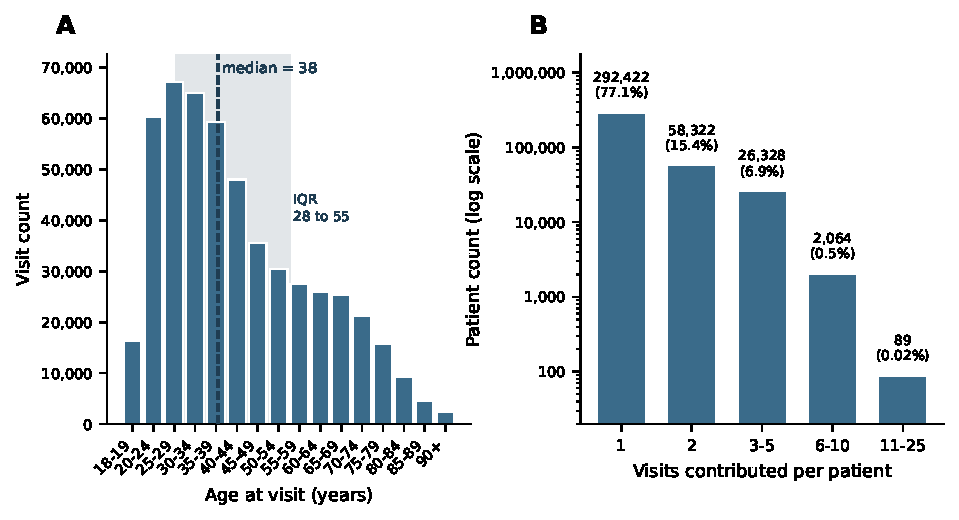
\includegraphics[width=\linewidth]{fig_demographics}
\end{center}
\caption{Demographic distribution of the analytic sample (n=514{,}381 visits from 379{,}227 unique patients). \textbf{(A)} Patient age distribution at the time of visit, binned in 5-year intervals; the distribution is right-skewed and peaks in the 25 to 29 bin. \textbf{(B)} Visits-per-patient distribution; 77.1\% of patients contributed a single visit and no patient contributed more than 25.}
\label{fig_demographics}
\end{figure}

\begin{figure}[h!]
\begin{center}
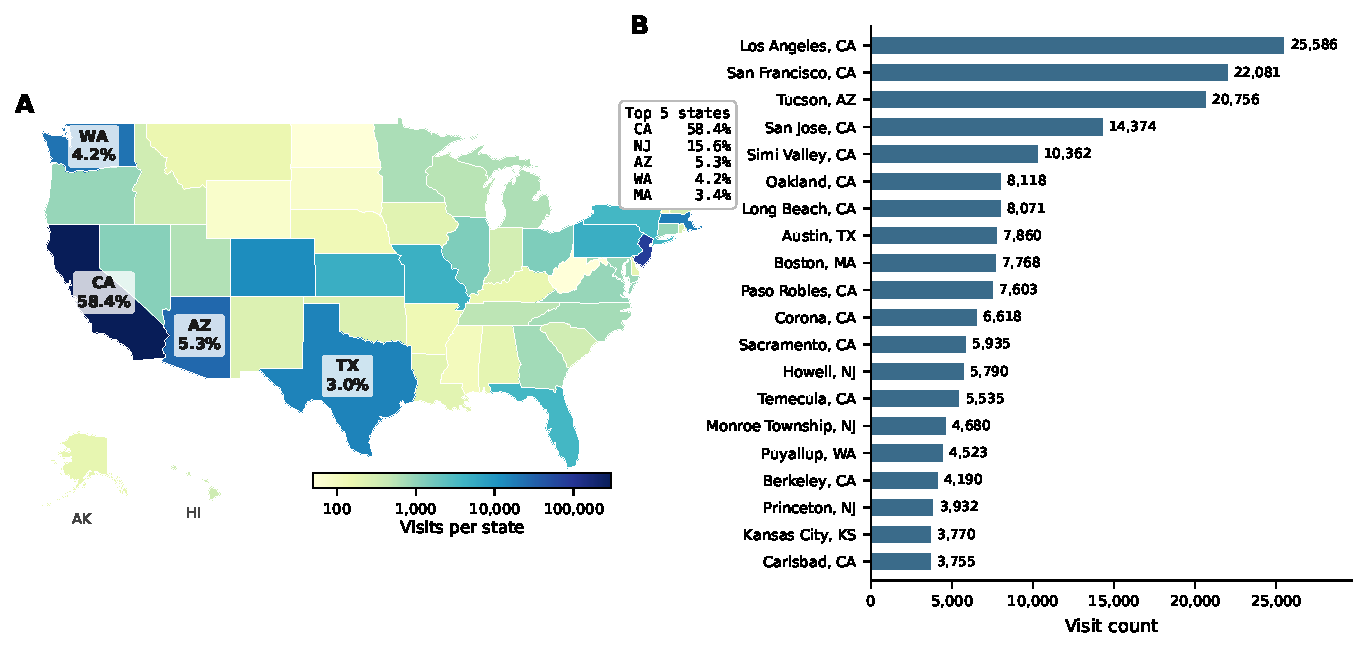
\includegraphics[width=\linewidth]{fig_geography}
\end{center}
\caption{Geographic distribution of the analytic sample (n=514{,}381 visits from 379{,}227 unique patients). \textbf{(A)} State-level visit counts; California accounts for 58.4\% of visits and the top five states (California, New Jersey, Arizona, Washington, Massachusetts) account for 86.9\%. \textbf{(B)} City-level visit distribution across 9{,}251 unique cities; the long tail comprises 3{,}800 cities (41\%) that contribute a single visit each.}
\label{fig_geography}
\end{figure}

\begin{figure}[h!]
\begin{center}
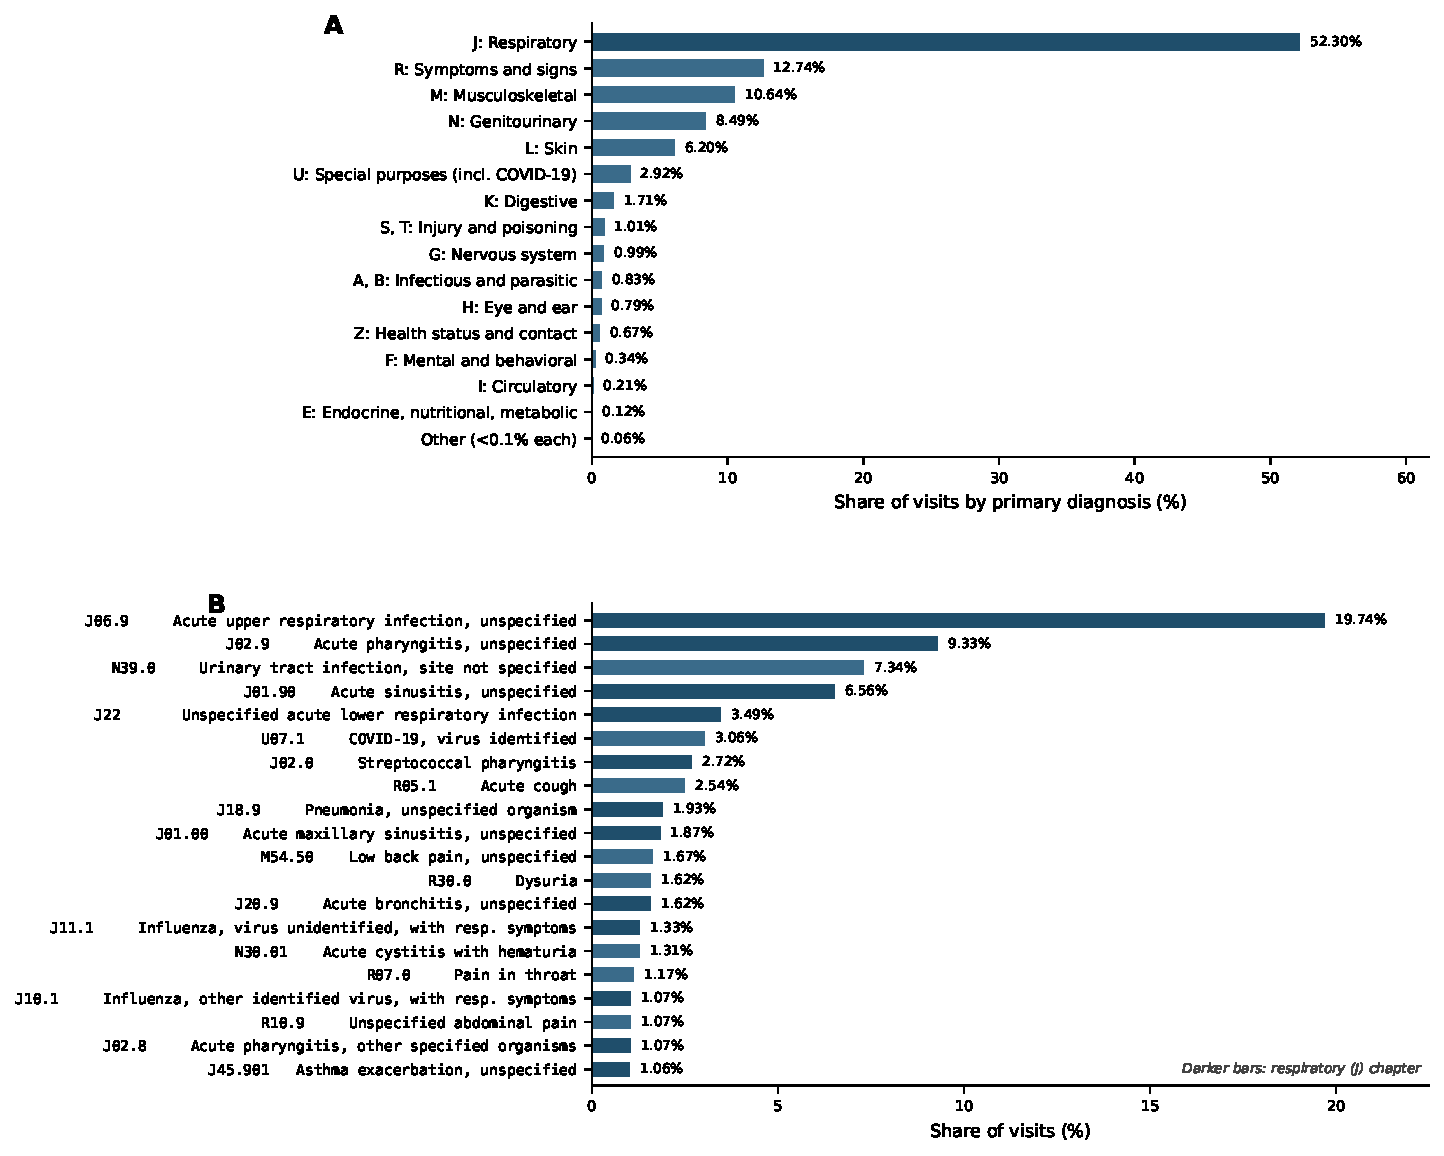
\includegraphics[width=\linewidth]{fig_clinical}
\end{center}
\caption{Clinical distribution of primary ICD-10 codes across the analytic sample (n=514{,}381 visits from 379{,}227 unique patients). \textbf{(A)} ICD-10 chapter distribution; the respiratory chapter (J) accounts for 52.3\% of primary diagnoses, followed by symptoms and signs (R, 12.74\%), musculoskeletal (M, 10.64\%), genitourinary (N, 8.49\%), and skin (L, 6.20\%). \textbf{(B)} Top primary ICD-10 codes; the top 20 codes account for 71.07\% of visits, led by J06.9 (acute upper respiratory infection, unspecified) at 19.74\% and J02.9 (acute pharyngitis, unspecified) at 9.33\%.}
\label{fig_clinical}
\end{figure}

\begin{figure}[h!]
\begin{center}
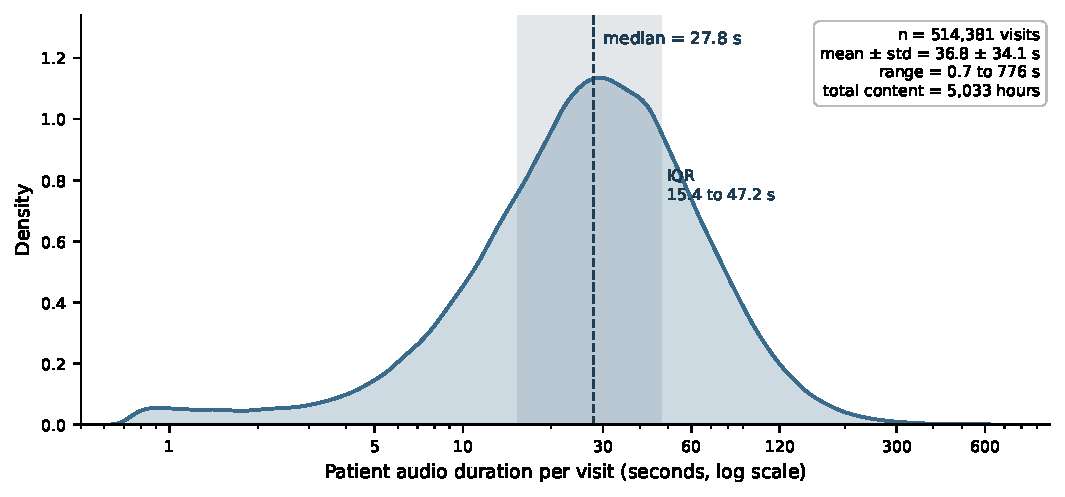
\includegraphics[width=\linewidth]{fig_duration}
\end{center}
\caption{Patient-channel audio duration across the analytic sample (n=514{,}381 visits). The distribution is unimodal and right-skewed on a linear scale (median 27.8 s, interquartile range 15.4 to 47.2 s, mean 36.8 $\pm$ 34.1 s, range 0.7 to 776 s); on the log scale shown here it appears roughly symmetric. The total measured patient audio is 5{,}033 hours.}
\label{fig_duration}
\end{figure}

\begin{figure}[h!]
\begin{center}
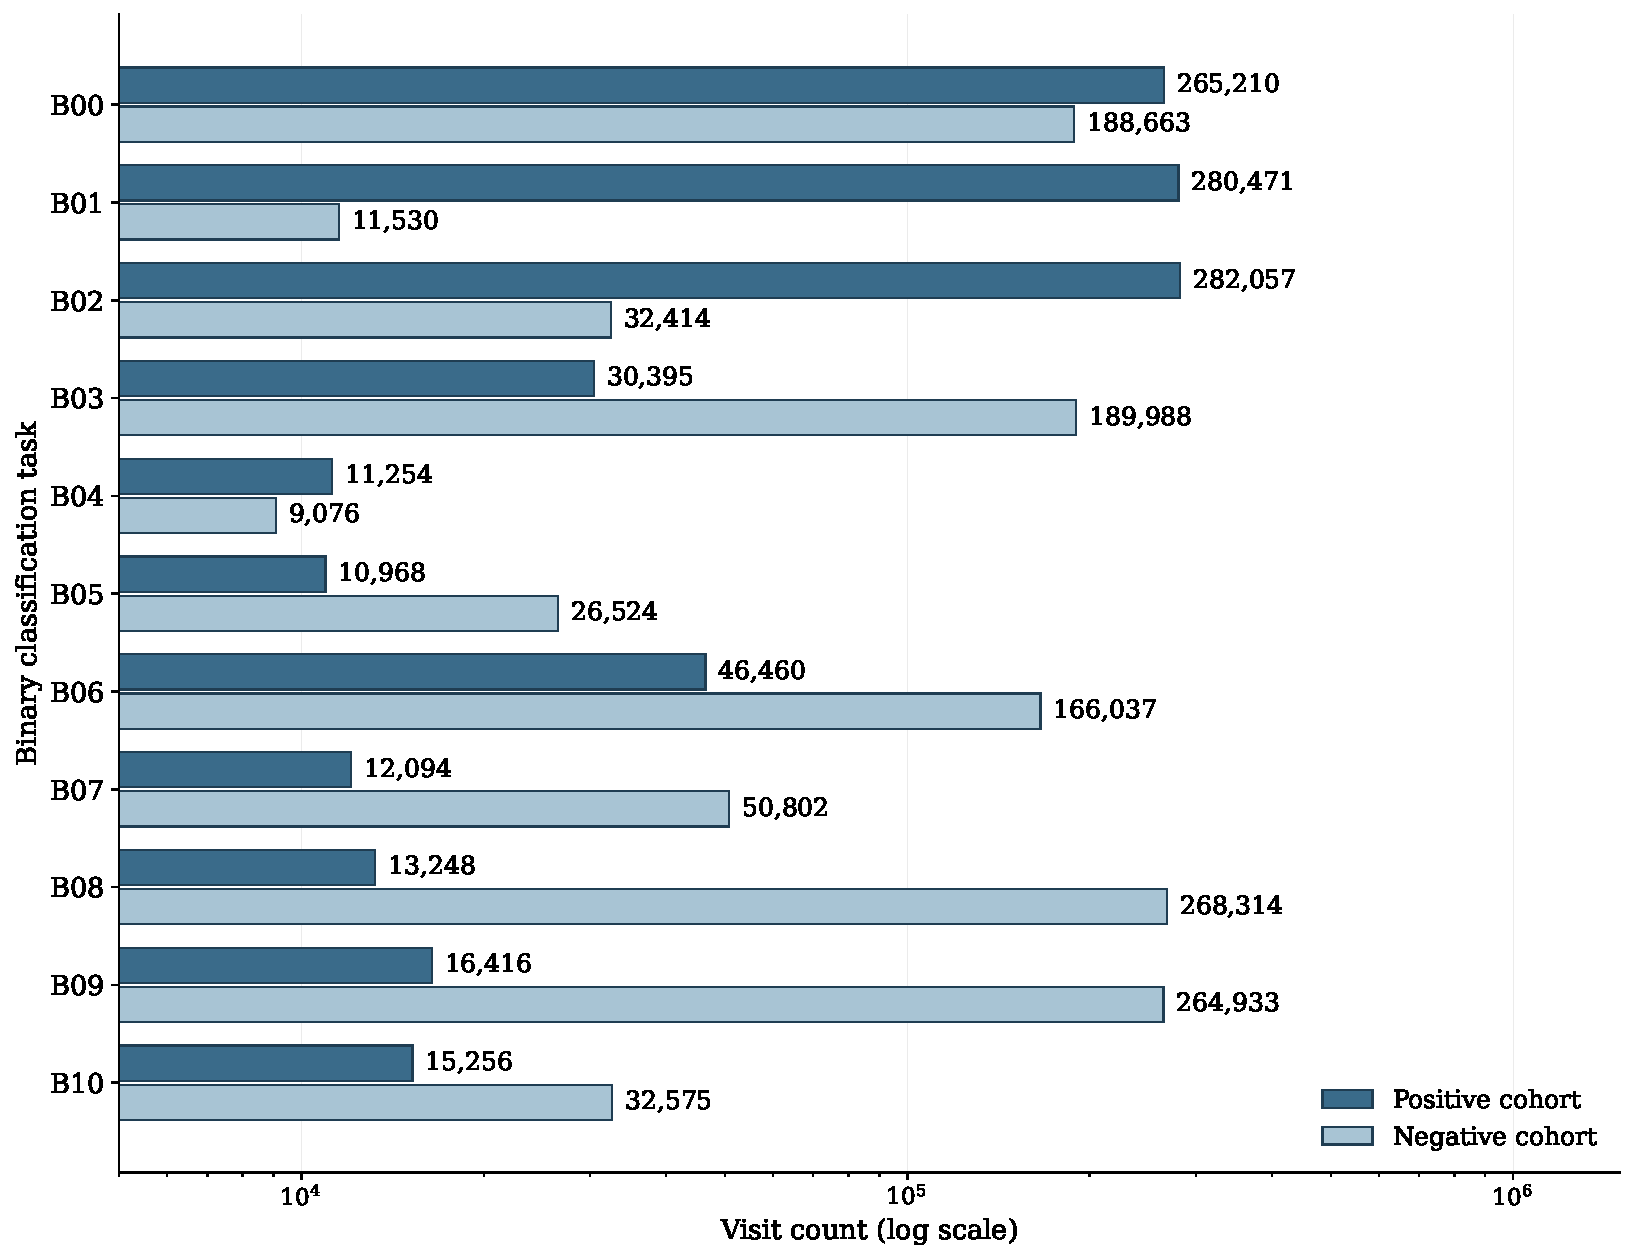
\includegraphics[width=\linewidth]{fig_cohort_sizes}
\end{center}
\caption{Per-task cohort sizes for the 11 binary classification tasks. Each task has a positive (label=1) and negative (label=0) cohort; sizes range from approximately 10{,}000 to 280{,}000 visits per class. Imbalance ratios reflect the natural prevalence of each clinical contrast in the source population, from near unity (B04, 1.24:1) to over 20:1 for B08 and B09.}
\label{fig_cohort_sizes}
\end{figure}

% --- Template example figure blocks below, kept for reference and commented out. ---
\iffalse
\begin{figure}[h!]
\begin{center}

\includegraphics[width=10cm]{logo1}% This is a *.eps file
\end{center}
\caption{ Enter the caption for your figure here.  Repeat as  necessary for each of your figures}\label{fig:1}
\end{figure}

\setcounter{figure}{2}
\setcounter{subfigure}{0}
\begin{subfigure}
\setcounter{figure}{2}
\setcounter{subfigure}{0}
    \centering
    \begin{minipage}[b]{0.5\textwidth}
        
\includegraphics[width=\linewidth]{logo1.eps}
        \caption{This is Subfigure 1.}
        \label{fig:Subfigure 1}
    \end{minipage}

\setcounter{figure}{2}
\setcounter{subfigure}{1}
    \begin{minipage}[b]{0.5\textwidth}
        
\includegraphics[width=\linewidth]{logo2.eps}
        \caption{This is Subfigure 2.}
        \label{fig:Subfigure 2}
    \end{minipage}

\setcounter{figure}{2}
\setcounter{subfigure}{-1}
    \caption{Enter the caption for your subfigure here. \textbf{(A)} This is the caption for Subfigure 1. \textbf{(B)} This is the caption for Subfigure 2.}
    \label{fig: subfigures}
\end{subfigure}
\fi

%%% If you don't add the figures in the LaTeX files, please upload them when submitting the article.
%%% Frontiers will add the figures at the end of the provisional pdf automatically
%%% The use of LaTeX coding to draw Diagrams/Figures/Structures should be avoided. They should be external callouts including graphics.

\end{document}
